\section{Design concepts and language support}

Our concepts provide a design-time support to build a software, considering
different situations it should adapt to and corresponding behavioral variations.
They are also helps to to identify the common functionality, orthogonal aspects
and mutual constraints.

\subsection{Concepts}\label{subsec:concepts}

Our approach includes such concepts as \emph{i) context}, \emph{ii) context
group} and a number of notions to build a complete design. Context represents an
environmental situation the system may find itself in, and defines a behavioral
variation for current situation. The software adapts to the environmental
dynamics by activating the corresponding context. Context group represents a
collection of contexts, which are representing the behavior variations of the
same functionality.

\begin{figure}
\begin{center}
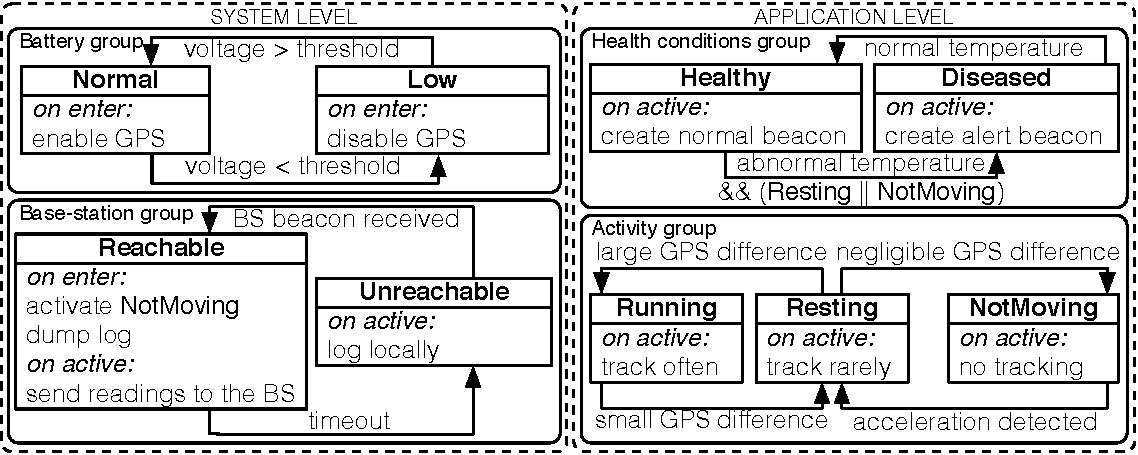
\includegraphics[scale=.45]{imgs/wildlifetracking}
\vspace{-4mm}
\caption{Wildlife monitoring application design.}
  \label{fig:design}
\vspace{-6mm}
\end{center}
\end{figure}

The context-oriented design of our motivating example is displayed in
Fig.~\ref{fig:design}. Context groups describe a behavioral variation
corresponding to battery level, base-station availability, health conditions and
activity of an animal. Notion of \emph{context group} allows us to separate
re-usable system services from application-specific functionality.

The context corresponds to the behavioral variation for a given situation. For
example, software behaves differently, depending on whether the base-station is
reachable or not. The contexts transitions within the group are governed by
rules. For example, within "Base-station'' group, the system initiates the
transition from "Reachable'' to "Unreachable'' whenever there are no beacons are
received within a specific timeout. In the "Unreachable'' context, the system
stores the contact logs locally.

In the specific context there is a distinction between \emph{one-time operation}
executed at the time of entering or exiting a context, and \emph{continuous
activities} that occurs as long as context is active. For example, in the latter
situation software logs contacts locally as long as "Unreachable'' context is
active, but dumps log on the base station on entering context "Reachable''.

The required adaptation may affect several context groups. For example, along
with the base-station is "Reachable'', context "NotMoving'' should be also
activated. The latter saves energy by disabling GPS-sensor, since the
base-station is static and deployed in the known location. Developers may also
want to check design error at run-time. The example is in "Health conditions''
group: when activating "Diseased'' context based on body temperature, the
software should also check that either "NotMoving'' or "Resting'' in "Activity
group'' is currently active. Indeed, a diseased animal is probably not very
active. Otherwise, developers might have not correctly understood how the
contexts evolve.

\subsection{Programming support}

To be more concrete in our design, we render the concepts above in a set of
language constructs, according to a context-oriented programming
(COP)~\cite{Hirschfeld08}. Our target language is nesC - one of the most popular
for programming for WSNs derived from C. Applications in nesC are built from
\emph{components} interconnected by \emph{configuration} and interacted by
\emph{using} and \emph{providing} interfaces. The latter define two types of
functions: \emph{commands} and \emph{events}.

nesC exemplifies the restrictions of CPSs such as limited memory and CPU
performance as well as absence of memory protection. Thus, the components can
not be instantiated at run-time, and dynamic allocation is also discouraging.
That is why COP can not be ported directly.

{\bfseries ConesC.} Taking into account restrictions above, we developed a
context-oriented extension of nesC language, called \conesc, that implements
concepts decribed in Section~\ref{subsec:concepts}.

The core notion is~\emph{layered function}~\cite{Hirschfeld08}, whose behavior
depends on activated context, and thus means to implement a behavioral
variation. A \emph{context group} in \conesc extends standard nesC configuration
by specifying contexts included and layered functions implemented in such
contexts. The latter are providing the context-dependent implementation of
layered functions.

\begin{figure}[!tb]
\begin{lstlisting}[style=conescframe]
context group BaseStationG {
*\lstnote{cg:layered}* layered command void report(contact_t contact);
}implementation {
*\lstnote{cg:ctx}* contexts Reachable, 
*\lstnote{cg:def}*          Unreachable is default,
*\lstnote{cg:error}*          ErrorC is error;
 // Standard nesC component wirings... }
\end{lstlisting}
\vspace{-5mm}
\caption{Context group in \conesc.}
  \label{fig:configuration}
\vspace{-3mm}
\end{figure}

The snippet of \conesc code implementing "Base Station'' group is displayed in
Figure~\ref{fig:configuration}. Here the function \code{report()} on
line~\lstref{cg:layered} behaves differently depending whether the base-station
\code{Reachable} or \code{Unreachable}. The latter are context included in the
group, declared on line~\lstref{cg:ctx}. The optional modifier \code{is error}
(line~\lstref{cg:error}) indicated an error context, while the modifier \code{is
default} (line~\lstref{cg:def}) specifies the active context at the start-up.
The former is automatically activated should the constraints be violated, e.g.,
when "Diseased'' is activated, "Resting'' or "NotMoving'' must be active, as
shown in Figure~\ref{fig:design}.

\begin{figure}[!tb]
\begin{lstlisting}[style=conescframe]
context Reachable {
*\lstnote{ct:tr}* transitions Unreachable;
*\lstnote{ct:trigger}* triggers NotMoving;
 uses interface Radio;
} implementation {
*\lstnote{ct:layer}* layered command void report(contact_t contact){
  call Radio.send(contact);}
*\lstnote{ct:activate}* event void activated(){// Dump logs on base-station }
*\lstnote{ct:deactivate}* event void deactivated(){ // Radio clean-up }}
\end{lstlisting}
\vspace{-5mm}
\caption{Individual context in \conesc.}
  \label{fig:context}
\vspace{-5mm}
\end{figure}

Specification of the "Reachable'' context is shown in Figure~\ref{fig:context}.
The keyword \code{triggers} on line~\lstref{ct:trigger} binds the activation
across the groups. For example, the context "NotMoving'' is activated on
entering the "Unreachable'', as specified in Figure~\ref{fig:design}. The
specific implementation of layered function is defined on line~\lstref{ct:layer}
by using a key-word \code{layered}. The one-time operations can be implemented
by using predefined events \code{activated()} and \code{deactivated()}, shown on
lines~\lstref{ct:activate} and~\lstref{ct:deactivate}. These events are
automatically signaled when entering or leaving the contexts. The contexts
indicated after the key-word \code{transitions} on line \lstref{ct:tr}
represents possible outgoing transitions. They are also possibly followed by a
key-word \code{iff} to state constraints on the transitions, as in

\begin{lstlisting}[language=conesc]
transitions Diseased iff Resting || NotMoving;
\end{lstlisting}

to encode a constraints in the definition of "Healthy''. Should the constraints
be violated, the error context defined in the corresponding context group is
activated. Explicit context activation can be initiated anywhere in the code, as
in

\begin{lstlisting}[language=conesc]
activate BaseStationG.Unreachable;
\end{lstlisting}
